\documentclass[10pt,a4paper]{article}

\usepackage[utf8]{inputenc}
\usepackage[T1]{fontenc}
\usepackage[spanish,es-nodecimaldot]{babel}
\usepackage[top=1.5cm, bottom=2cm, left=1.5cm, right=1.5cm]{geometry}
\usepackage{setspace}
\singlespacing
\usepackage{graphicx}
\usepackage{float}
\usepackage{booktabs}
\usepackage{array}
\usepackage{tabularx}
\usepackage{hyperref}
\usepackage{xcolor}
\usepackage{amsmath}
\usepackage{caption}
\usepackage{listings}
\usepackage{parskip}
\usepackage[round,authoryear]{natbib}
\usepackage{fancyhdr}

\definecolor{codebackground}{HTML}{F5F5F5}
\definecolor{codecomment}{HTML}{6A9955}
\definecolor{codestring}{HTML}{CE9178}
\definecolor{codekeyword}{HTML}{569CD6}
\definecolor{headerdark}{HTML}{2C3E50}

\setlength{\parskip}{3pt}
\setlength{\textfloatsep}{8pt plus 1pt minus 2pt}
\setlength{\floatsep}{6pt plus 1pt minus 2pt}
\setlength{\intextsep}{6pt plus 1pt minus 2pt}
\renewcommand{\arraystretch}{0.95}

\lstset{
  language=R,
  backgroundcolor=\color{codebackground},
  basicstyle=\ttfamily\footnotesize,
  breaklines=true,
  frame=single,
  rulecolor=\color{gray!40},
  commentstyle=\color{codecomment},
  stringstyle=\color{codestring},
  keywordstyle=\color{codekeyword}\bfseries,
  numbers=left,
  numberstyle=\tiny\color{gray},
  numbersep=5pt,
  tabsize=2,
  showstringspaces=false,
  captionpos=b
}

\hypersetup{
  colorlinks=true,
  linkcolor=headerdark,
  citecolor=headerdark,
  urlcolor=blue!70!black,
  pdftitle={Analisis de Componentes Principales del Dataset Boston},
  pdfauthor={Vicente Rivera, Juan Munoz, Fernando Valdes}
}

\captionsetup{font=small, labelfont=bf}

\begin{document}

\begin{center}
  {\large \textbf{Universidad Catolica de Temuco}} \\[2pt]
  {\normalsize Facultad de Ingenieria -- INFO1184 Inteligencia de Negocios} \\[6pt]
  \rule{0.86\textwidth}{0.6pt} \\[6pt]
  {\Large \textbf{TAREA 04}} \\[3pt]
  {\LARGE \textbf{Analisis de Componentes Principales}} \\[3pt]
  {\LARGE \textbf{Dataset Boston -- Metodologia CRISP-DM}} \\[8pt]
  {\normalsize \textbf{Docente:} Marcos Levano Humacto} \\[2pt]
  {\normalsize \textbf{Desarrollado por:} Vicente Rivera, Juan Mu\~noz, Fernando Valdes} \\[2pt]
  {\small vrivera2023@alu.uct.cl, juan.munozveloso2023@alu.uct.cl, fvaldes2023@alu.uct.cl} \\[2pt]
  {\small Tarea 4, INFO1184, Semestre I-2026} \\[6pt]
  \rule{0.86\textwidth}{0.6pt}
\end{center}

\section*{Resumen}

Este informe aplica Analisis de Componentes Principales (PCA) al dataset \texttt{Boston}, disponible en el paquete \texttt{MASS} de R, siguiendo las fases principales de CRISP-DM. El conjunto contiene 506 observaciones y 14 variables asociadas a criminalidad, uso de suelo, contaminacion, accesibilidad, condicion socioeconomica y valor mediano de viviendas. Se revisaron valores faltantes, outliers por regla IQR y relaciones entre precio, habitaciones, condicion de limitar con el rio Charles y estatus socioeconomico. El PCA permitio sintetizar la estructura multivariada: cinco componentes explicaron el 80,58\% de la varianza total. Los resultados directos muestran correlacion positiva entre \texttt{rm} y \texttt{medv} (0,695), correlacion negativa entre \texttt{lstat} y \texttt{medv} (-0,738), y una diferencia media de 6,346 miles de dolares a favor de sectores que limitan con el rio Charles ($p = 0,00357$). Para criminalidad, una regresion lineal sobre componentes principales predijo \texttt{log1p(crim)} con $R^{2} = 0,8119$ y mejora de 11,85\% en RMSE frente al promedio base. El analisis es reproducible y exploratorio.

\textbf{Palabras clave:} PCA, CRISP-DM, Boston, vivienda, criminalidad, R Project.

\section{Introduccion}

La inteligencia de negocios aplicada al analisis urbano permite convertir datos historicos en informacion para comprender precios de viviendas, condiciones del entorno y riesgos territoriales. El dataset \texttt{Boston} reune variables de suburbios del area de Boston relacionadas con criminalidad, uso de suelo, contaminacion, accesibilidad, educacion, estatus socioeconomico y valor mediano de viviendas \citep{harrison1978, venables2002}.

El objetivo de la tarea es usar PCA dentro de CRISP-DM para responder seis preguntas: existencia de valores atipicos; observaciones con casas mas baratas; influencia del tamano de la vivienda; efecto de limitar con el rio Charles; impacto del estatus socioeconomico; y posibilidad de predecir criminalidad. El informe conserva los resultados cuantitativos principales en el cuerpo y deja visualizaciones, tablas secundarias y procedimientos de R en el anexo.

\section{Fundamentos Teoricos}

CRISP-DM (\textit{Cross-Industry Standard Process for Data Mining}) organiza proyectos de mineria de datos en comprension del negocio, comprension de datos, preparacion, modelamiento, evaluacion y despliegue \citep{chapman2000}. En esta tarea se desarrollan las fases 1 a 5, porque el objetivo es analitico y no contempla implementacion productiva.

PCA transforma variables posiblemente correlacionadas en componentes ortogonales ordenados por varianza explicada \citep{jolliffe2002}. Dado que las variables estan en escalas distintas, primero se estandariza cada valor mediante z-score:

\begin{equation}
  z_{ij} = \frac{x_{ij} - \bar{x}_j}{s_j},
\end{equation}

donde $x_{ij}$ es el valor de la observacion $i$ en la variable $j$, $\bar{x}_j$ es su media y $s_j$ su desviacion estandar. Luego, sobre la matriz estandarizada $\mathbf{Z}$, se analiza la matriz de correlaciones $\mathbf{R}$ y sus autovalores:

\begin{equation}
  \mathbf{R}=\frac{1}{n-1}\mathbf{Z}^{\top}\mathbf{Z}, \qquad
  \mathbf{R}\mathbf{a}_k = \lambda_k\mathbf{a}_k.
\end{equation}

El componente $k$ para la observacion $i$ es una combinacion lineal de las variables estandarizadas:

\begin{equation}
  PC_{ik}=\mathbf{z}_i^{\top}\mathbf{a}_k=\sum_{j=1}^{p} a_{jk}z_{ij}, \qquad
  \text{Varianza explicada}_k=\frac{\lambda_k}{\sum_{l=1}^{p}\lambda_l}.
\end{equation}

Para evaluar la prediccion de criminalidad se uso regresion lineal sobre componentes principales y la variable objetivo \texttt{log1p(crim)}. El desempeno se reporta con RMSE y $R^{2}$:

\begin{equation}
  RMSE = \sqrt{\frac{1}{n}\sum_{i=1}^{n}(y_i - \hat{y}_i)^2}, \qquad
  R^{2} = 1 - \frac{\sum_{i=1}^{n}(y_i - \hat{y}_i)^2}{\sum_{i=1}^{n}(y_i - \bar{y})^2}.
\end{equation}

\section{Desarrollo}

\subsection{Fases 1 a 3: negocio, datos y preparacion}

El problema de negocio consiste en identificar condiciones urbanas y socioeconomicas asociadas al precio de viviendas y a la criminalidad. Como criterio de exito se exigio que cada pregunta quedara respaldada por una evidencia directa y, cuando fuera pertinente, por la lectura multivariada del PCA.

El dataset contiene 506 observaciones y 14 variables numericas, sin valores faltantes. La variable \texttt{medv} presenta media 22,533 y rango 5 a 50; \texttt{crim} tiene media 3,614, mediana 0,257 y maximo 88,976, lo que evidencia asimetria. La variable \texttt{black} se conserva por reproducibilidad del dataset original, pero por su origen historico y sensibilidad interpretativa no se usa para conclusiones sociales sustantivas.

\begin{table}[H]
  \centering
  \caption{Sintesis de datos, preparacion y evidencia exploratoria principal.}
  \label{tab:sintesis_datos}
  \footnotesize
  \begin{tabularx}{\textwidth}{p{3.1cm} X}
    \toprule
    \textbf{Aspecto} & \textbf{Resultado usado en el analisis} \\
    \midrule
    Estructura & 506 observaciones y 14 variables originales del dataset \texttt{Boston}. \\
    Calidad de datos & No se detectaron valores faltantes; las variables se estandarizaron con \texttt{prcomp(center = TRUE, scale. = TRUE)}. \\
    Outliers IQR & Mayores conteos en \texttt{black} (77), \texttt{zn} (68), \texttt{crim} (66), \texttt{medv} (40) y \texttt{rm} (30). \\
    Relaciones clave & \texttt{rm}-\texttt{medv}: 0,695; \texttt{lstat}-\texttt{medv}: -0,738; diferencia por \texttt{chas}: 6,346 miles de dolares. \\
    Preparacion predictiva & Para predecir \texttt{crim}, esta variable se separo como objetivo; el PCA predictivo uso las restantes variables y una division 70\% entrenamiento / 30\% prueba. \\
    \bottomrule
  \end{tabularx}
\end{table}

\subsection{Fase 4: modelamiento PCA}

El PCA exploratorio se aplico sobre las 14 variables estandarizadas: \texttt{crim}, \texttt{zn}, \texttt{indus}, \texttt{chas}, \texttt{nox}, \texttt{rm}, \texttt{age}, \texttt{dis}, \texttt{rad}, \texttt{tax}, \texttt{ptratio}, \texttt{black}, \texttt{lstat} y \texttt{medv}. Los cinco primeros componentes explicaron 80,58\% de la varianza total (Tabla~\ref{tab:pca_varianza}).

\begin{table}[H]
  \centering
  \caption{Varianza explicada por los primeros componentes principales.}
  \label{tab:pca_varianza}
  \footnotesize
  \begin{tabular}{l r r}
    \toprule
    \textbf{Componente} & \textbf{Varianza individual} & \textbf{Varianza acumulada} \\
    \midrule
    PC1 & 46,76\% & 46,76\% \\
    PC2 & 11,78\% & 58,54\% \\
    PC3 & 9,64\% & 68,17\% \\
    PC4 & 6,33\% & 74,51\% \\
    PC5 & 6,08\% & 80,58\% \\
    \bottomrule
  \end{tabular}
\end{table}

PC1 se interpreta como eje de presion urbana y socioeconomica: \texttt{indus} (0,3319), \texttt{nox} (0,3252), \texttt{tax} (0,3240), \texttt{lstat} (0,3114) y \texttt{rad} (0,3034) cargan positivamente, mientras \texttt{dis} (-0,2982), \texttt{medv} (-0,2666) y \texttt{zn} (-0,2454) aparecen en sentido contrario. PC2 opera como eje residencial asociado a \texttt{medv} (0,4449), \texttt{rm} (0,4340) y \texttt{chas} (0,4107), frente a cargas negativas como \texttt{dis} (-0,3591), \texttt{ptratio} (-0,3146) y \texttt{lstat} (-0,2012). La Figura~\ref{fig:pca_biplot_simple} muestra una version simplificada del biplot; la version completa queda en el anexo.

\begin{figure}[H]
  \centering
  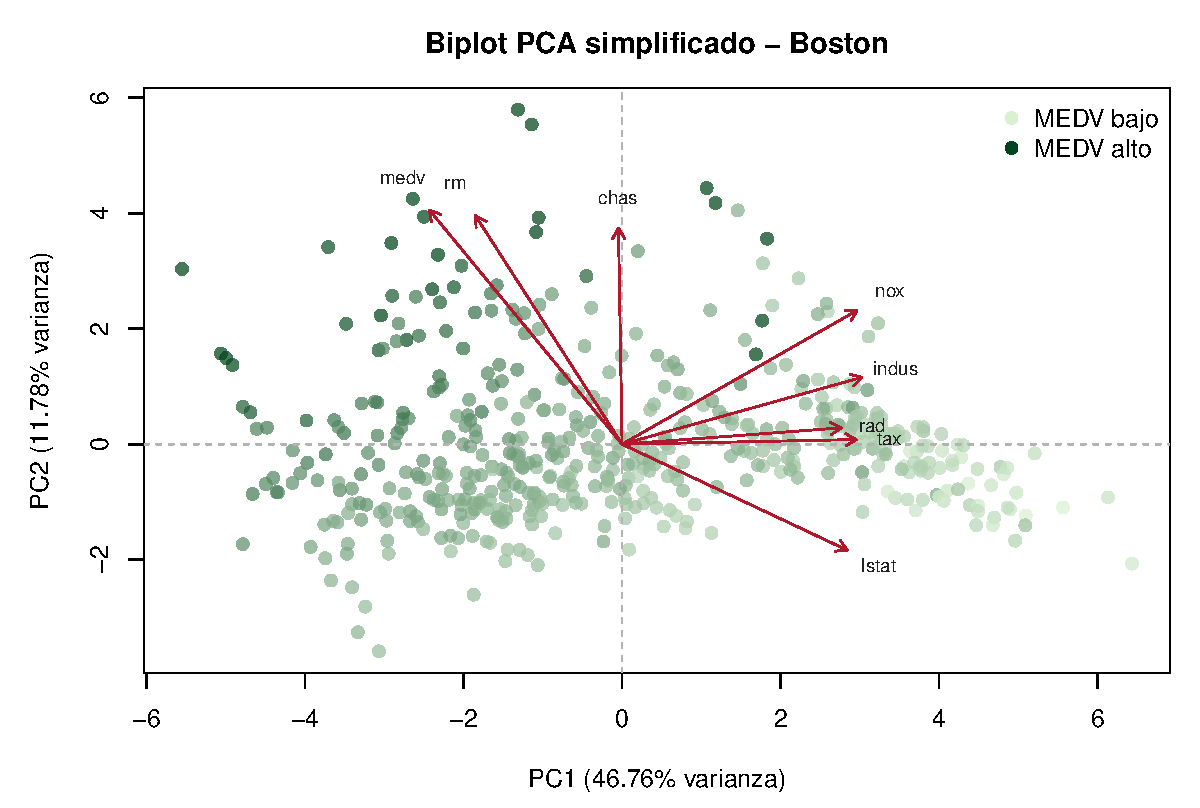
\includegraphics[width=0.68\textwidth]{figuras/fig_08_pca_biplot_simple.pdf}
  \caption{Biplot PCA simplificado con variables principales para interpretar PC1 y PC2.}
  \label{fig:pca_biplot_simple}
\end{figure}

\subsection{Fase 5: evaluacion y respuestas de investigacion}

La Tabla~\ref{tab:resumen_preguntas} integra las seis preguntas con su evidencia directa y su relacion con PCA. En la pregunta 2 se reportan observaciones mediante \texttt{id\_suburbio}, porque \texttt{Boston} no trae nombres reales de suburbios.

\begin{table}[H]
  \centering
  \caption{Respuestas de investigacion, evidencias y aporte del PCA.}
  \label{tab:resumen_preguntas}
  \footnotesize
  \begin{tabularx}{\textwidth}{p{2.2cm} X X}
    \toprule
    \textbf{Pregunta} & \textbf{Respuesta central y evidencia directa} & \textbf{Relacion con PCA} \\
    \midrule
    P1 Outliers & Si. Por IQR destacan \texttt{black} (77), \texttt{zn} (68), \texttt{crim} (66), \texttt{medv} (40) y \texttt{rm} (30). \texttt{black} solo se reporta por reproducibilidad. & \texttt{crim}, \texttt{zn}, \texttt{medv} y \texttt{rm} participan en PC1 o PC2, por lo que los extremos afectan ejes relevantes. \\
    P2 Casas mas baratas & El dataset no incluye nombres reales; se usan IDs internos. Los menores valores son ID 399 e ID 406 con \texttt{medv = 5}, luego ID 401 con 5,6 e ID 400 con 6,3; los diez casos mas baratos no limitan con el rio Charles. & \texttt{medv} se opone a PC1 y se alinea con PC2, ubicando estos casos en sentido contrario al mayor valor habitacional. \\
    P3 Tamano y precio & La relacion es positiva: correlacion \texttt{rm}-\texttt{medv} = 0,695; la regresion estima 9,102 miles de dolares adicionales por habitacion promedio ($p < 0,001$). & \texttt{rm} y \texttt{medv} cargan positivamente en PC2, reforzando la direccion residencial. \\
    P4 Rio Charles & Si, con cautela. La media de \texttt{medv} es 22,094 sin rio y 28,440 con rio; diferencia = 6,346 y $p = 0,00357$. \texttt{chas} es binaria y solo 35 de 506 observaciones limitan con el rio. & \texttt{chas} carga positivamente en PC2 junto con \texttt{medv}, coherente con la diferencia media observada. \\
    P5 Estatus & El impacto es negativo: correlacion \texttt{lstat}-\texttt{medv} = -0,738; cada punto adicional de \texttt{lstat} se asocia con -0,950 miles de dolares en \texttt{medv} ($p < 0,001$). & \texttt{lstat} y \texttt{medv} aparecen en direcciones opuestas en PC1 y PC2. \\
    P6 Criminalidad & Si, de forma exploratoria. Con 5 componentes se explico 82,84\% de la varianza de predictores; en prueba se obtuvo $R^{2} = 0,8119$ sobre \texttt{log1p(crim)} y mejora RMSE = 11,85\%. & El PCA resume predictores urbanos y socioeconomicos sin incluir \texttt{crim}; el split 70/30 puede variar segun semilla, por lo que un uso real requiere validacion cruzada o evaluacion adicional. \\
    \bottomrule
  \end{tabularx}
\end{table}

\section{Discusion y Reflexion}

CRISP-DM permitio ordenar el trabajo desde la definicion de preguntas hasta la evaluacion. El PCA fue util porque el dataset contiene variables redundantes: industrializacion, contaminacion, impuestos, accesibilidad radial y menor estatus socioeconomico se agrupan en PC1, mientras el valor habitacional aparece en direccion contraria. Esto entrega una lectura multivariada mas clara que revisar cada variable por separado.

Los resultados sobre precio son consistentes entre tecnicas: mas habitaciones se asocian con mayor \texttt{medv}, mayor \texttt{lstat} se asocia con menor \texttt{medv}, y limitar con el rio Charles muestra una diferencia positiva pero dependiente de una variable binaria con grupo reducido. En criminalidad, la transformacion \texttt{log1p} y los componentes principales mejoran la prediccion exploratoria, aunque el dataset es historico y no debe usarse directamente para decisiones actuales.

La principal precaucion metodologica es que el analisis describe asociaciones, no causalidad. Ademas, variables sensibles como \texttt{black} exigen una lectura etica: se mantienen para reproducibilidad, pero no fundamentan conclusiones sociales sustantivas. Para una aplicacion real se requeririan datos actualizados, revision de sesgos, validacion cruzada y comparacion con modelos no lineales.

\section{Conclusiones por Integrante}

\textbf{Vicente Rivera:} La revision inicial confirmo 506 observaciones, 14 variables y ausencia de faltantes, pero tambien outliers relevantes en \texttt{zn}, \texttt{crim}, \texttt{medv} y \texttt{rm}. Estos extremos importan porque aparecen en los ejes PC1 y PC2, por lo que la deteccion IQR no fue un paso aislado, sino parte de la interpretacion multivariada.

\textbf{Juan Mu\~noz:} CRISP-DM ayudo a conectar preguntas, evidencia y PCA. El resultado central fue que cinco componentes explicaron 80,58\% de la varianza; PC1 resume presion urbana/socioeconomica y se opone a \texttt{medv}, lo que respalda la lectura de menor valor en contextos con mayor carga urbana.

\textbf{Fernando Valdes:} La implementacion en R fue reproducible y mantuvo el codigo fuera del cuerpo del informe. Las evidencias mas fuertes fueron la relacion \texttt{rm}-\texttt{medv} (0,695), \texttt{lstat}-\texttt{medv} (-0,738) y el modelo de criminalidad con $R^{2} = 0,8119$ en escala logaritmica, utiles como resultados exploratorios y no como sistema operativo final.

\section{Referencias}
\small
\begin{thebibliography}{9}

\bibitem[Chapman et~al.(2000)]{chapman2000}
Chapman, P., Clinton, J., Kerber, R., Khabaza, T., Reinartz, T., Shearer, C., \& Wirth, R. (2000).
\textit{CRISP-DM 1.0: Step-by-step data mining guide}. SPSS Inc.

\bibitem[Harrison y Rubinfeld(1978)]{harrison1978}
Harrison, D., \& Rubinfeld, D. L. (1978).
Hedonic housing prices and the demand for clean air.
\textit{Journal of Environmental Economics and Management}, \textit{5}(1), 81--102.
\url{https://doi.org/10.1016/0095-0696(78)90006-2}

\bibitem[Jolliffe(2002)]{jolliffe2002}
Jolliffe, I. T. (2002).
\textit{Principal component analysis} (2nd ed.). Springer.
\url{https://doi.org/10.1007/b98835}

\bibitem[R Core Team(2024)]{rcore2024}
R Core Team. (2024).
\textit{R: A language and environment for statistical computing}. R Foundation for Statistical Computing.
\url{https://www.R-project.org/}

\bibitem[Venables y Ripley(2002)]{venables2002}
Venables, W. N., \& Ripley, B. D. (2002).
\textit{Modern applied statistics with S} (4th ed.). Springer.
\url{https://doi.org/10.1007/978-0-387-21706-2}

\end{thebibliography}

\newpage
\section*{Anexo}
\addcontentsline{toc}{section}{Anexo}

\subsection*{A.1 Visualizaciones Complementarias}

\begin{figure}[H]
\centering
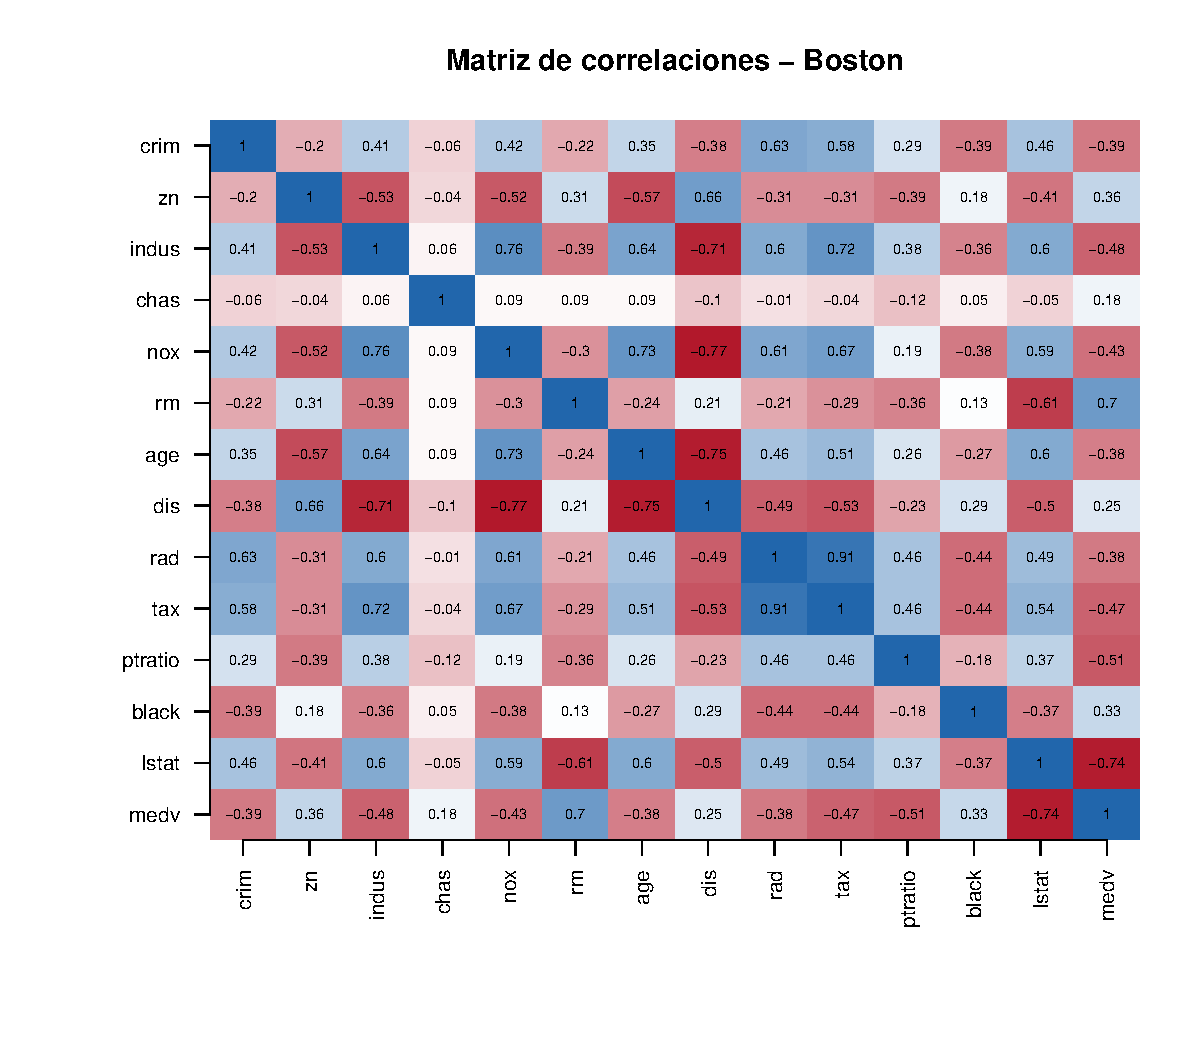
\includegraphics[width=0.72\textwidth]{figuras/fig_01_matriz_correlaciones.pdf}
\caption{Matriz de correlaciones entre variables del dataset Boston.}
\label{fig:correlaciones}
\end{figure}

\begin{figure}[H]
\centering
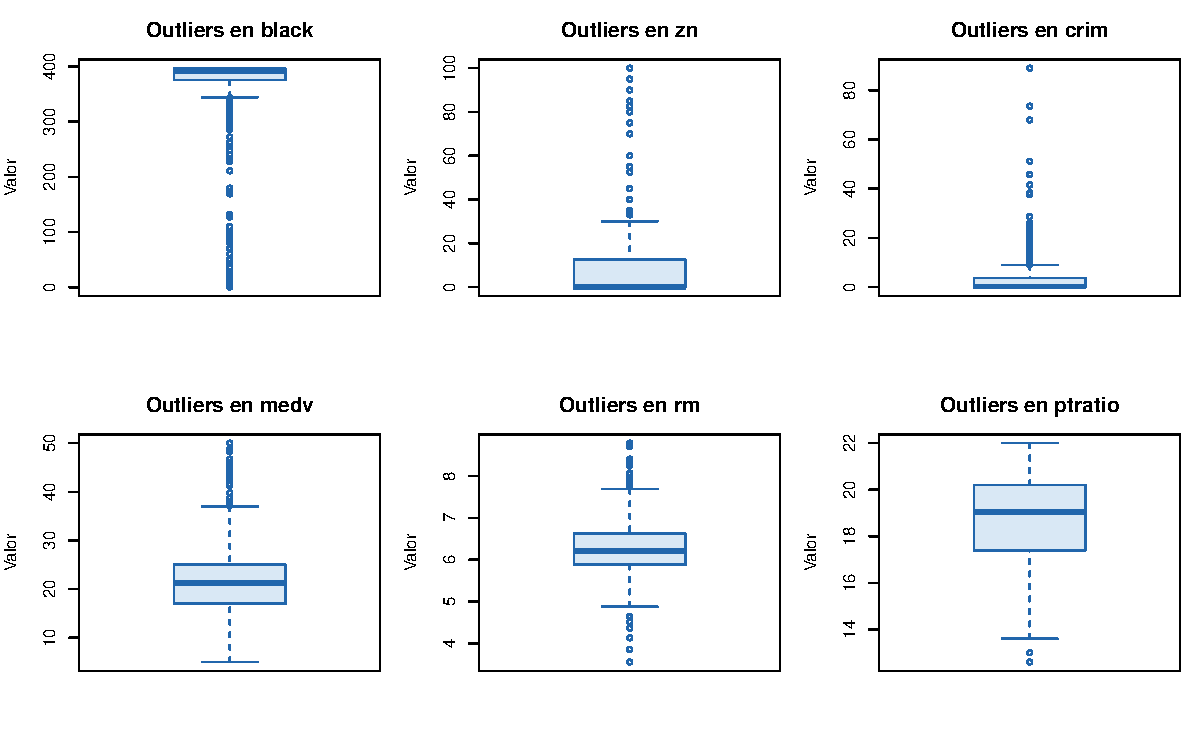
\includegraphics[width=0.85\textwidth]{figuras/fig_02_outliers_boxplot.pdf}
\caption{Variables con mayor cantidad de valores atipicos segun regla IQR.}
\label{fig:outliers}
\end{figure}

\begin{figure}[H]
\centering
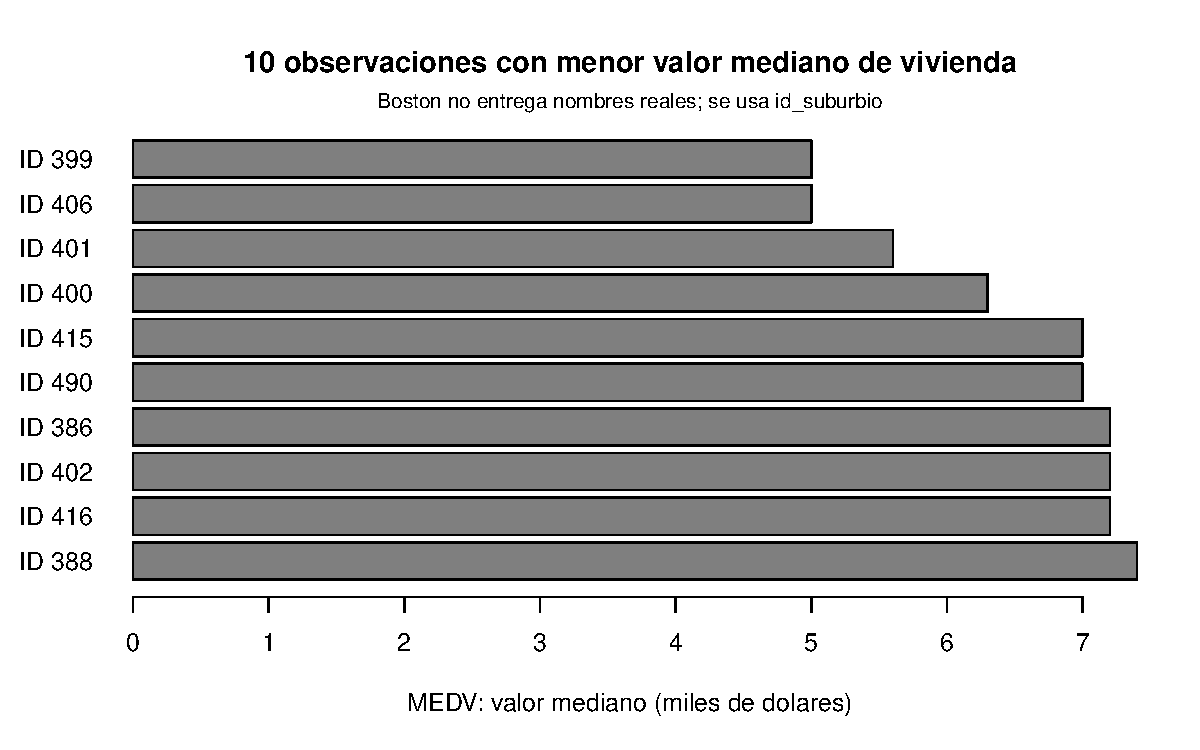
\includegraphics[width=0.82\textwidth]{figuras/fig_03_suburbios_mas_baratos.pdf}
\caption{Diez observaciones del dataset con menor valor mediano de vivienda.}
\label{fig:baratos}
\end{figure}

\begin{figure}[H]
\centering
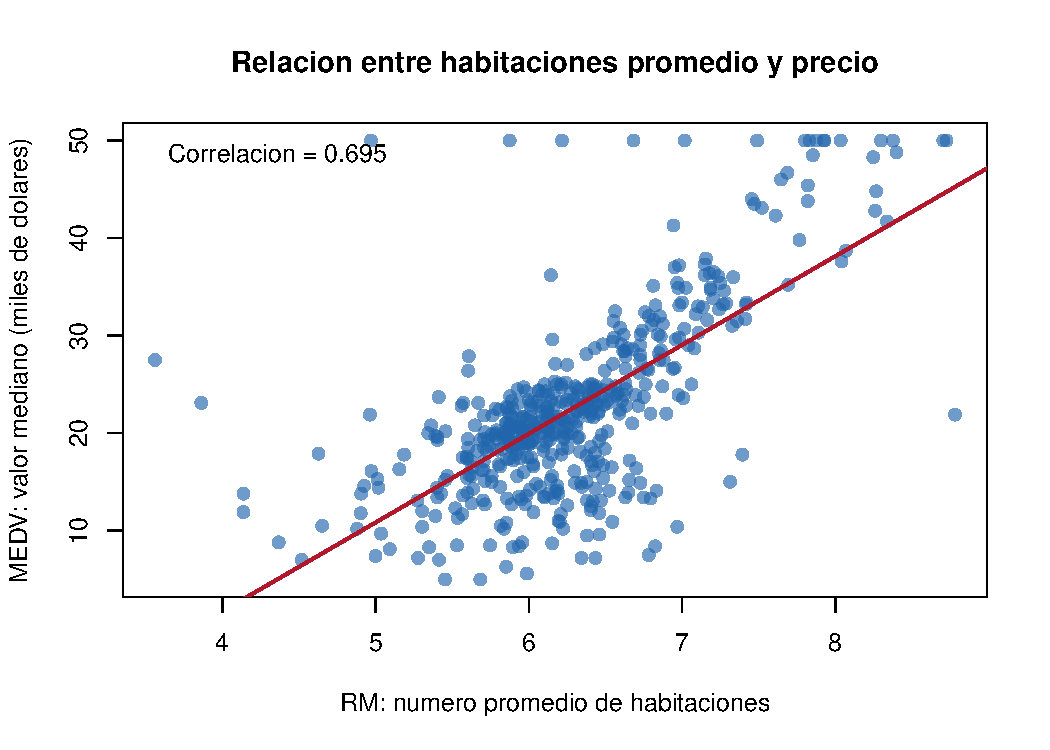
\includegraphics[width=0.72\textwidth]{figuras/fig_04_rm_vs_medv.pdf}
\caption{Relacion entre habitaciones promedio y valor mediano de vivienda.}
\label{fig:rm_medv}
\end{figure}

\begin{figure}[H]
\centering
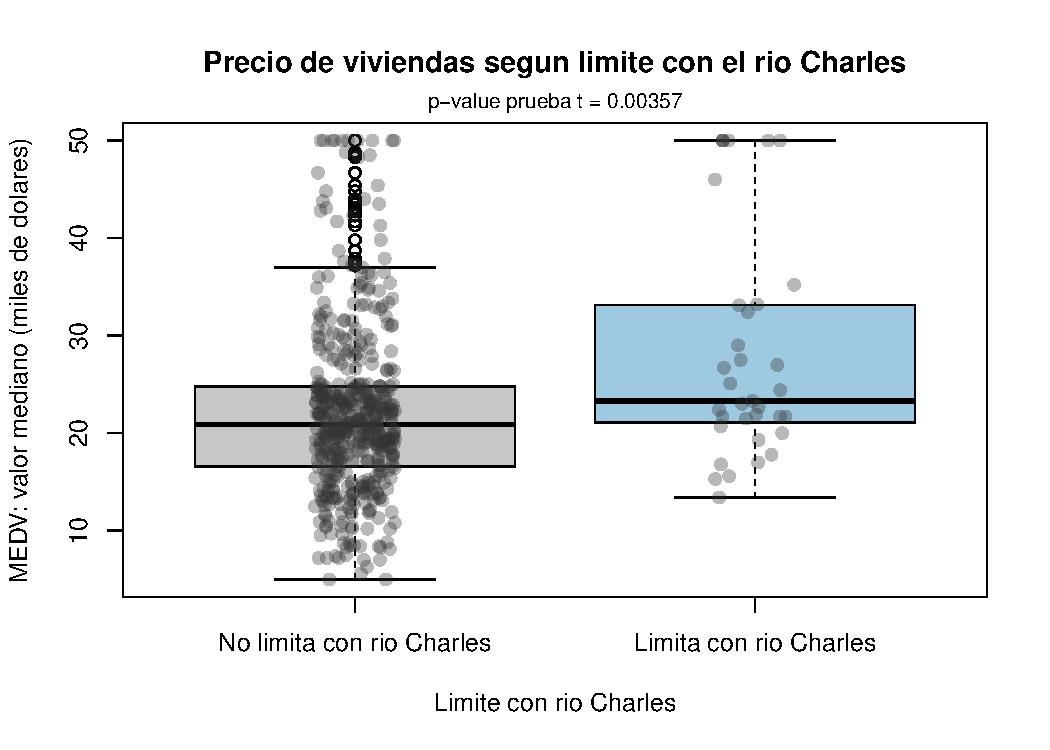
\includegraphics[width=0.72\textwidth]{figuras/fig_05_chas_vs_medv.pdf}
\caption{Valor mediano de viviendas segun limite con el rio Charles.}
\label{fig:chas_medv}
\end{figure}

\begin{figure}[H]
\centering
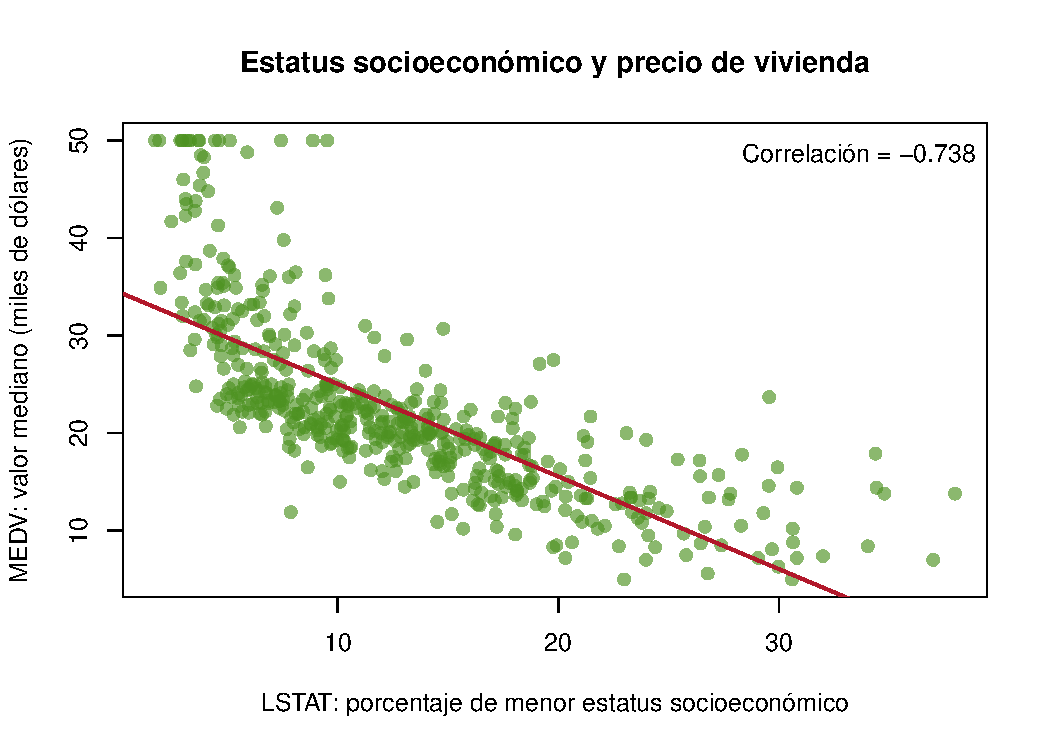
\includegraphics[width=0.72\textwidth]{figuras/fig_06_lstat_vs_medv.pdf}
\caption{Relacion entre estatus socioeconomico y valor mediano de vivienda.}
\label{fig:lstat_medv}
\end{figure}

\begin{figure}[H]
\centering
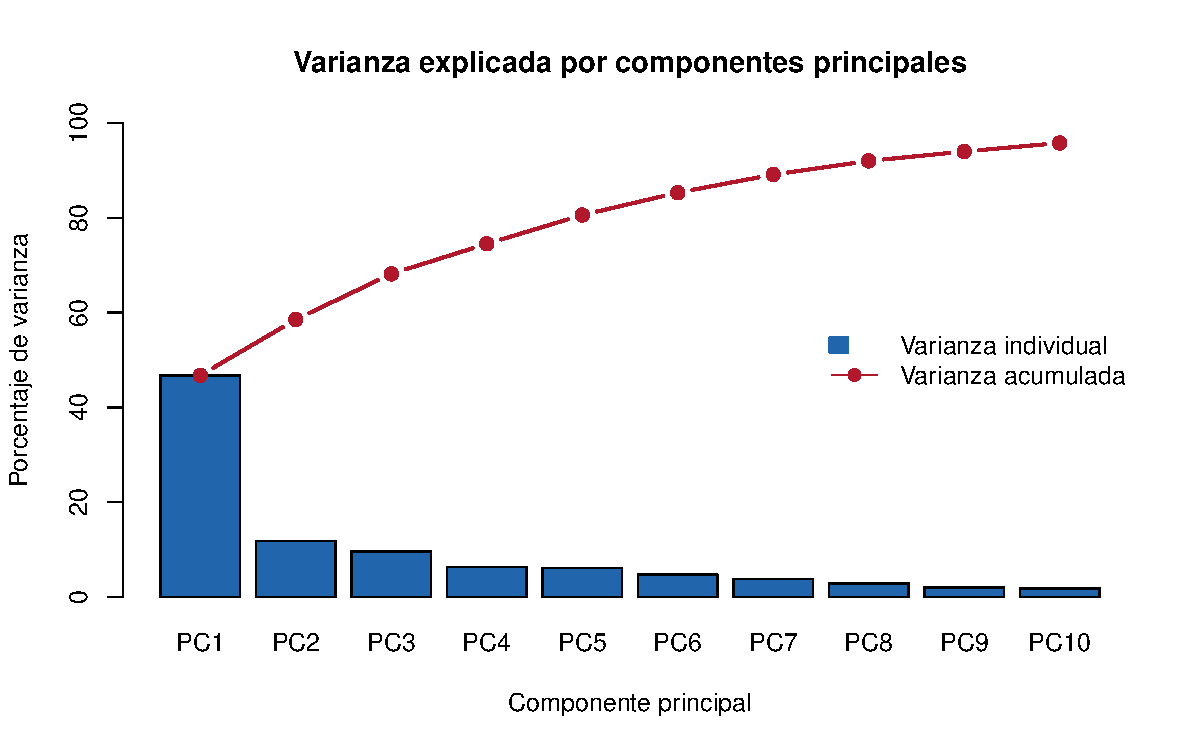
\includegraphics[width=0.72\textwidth]{figuras/fig_07_pca_varianza_explicada.pdf}
\caption{Varianza individual y acumulada explicada por los componentes principales.}
\label{fig:pca_varianza}
\end{figure}

\begin{figure}[H]
\centering
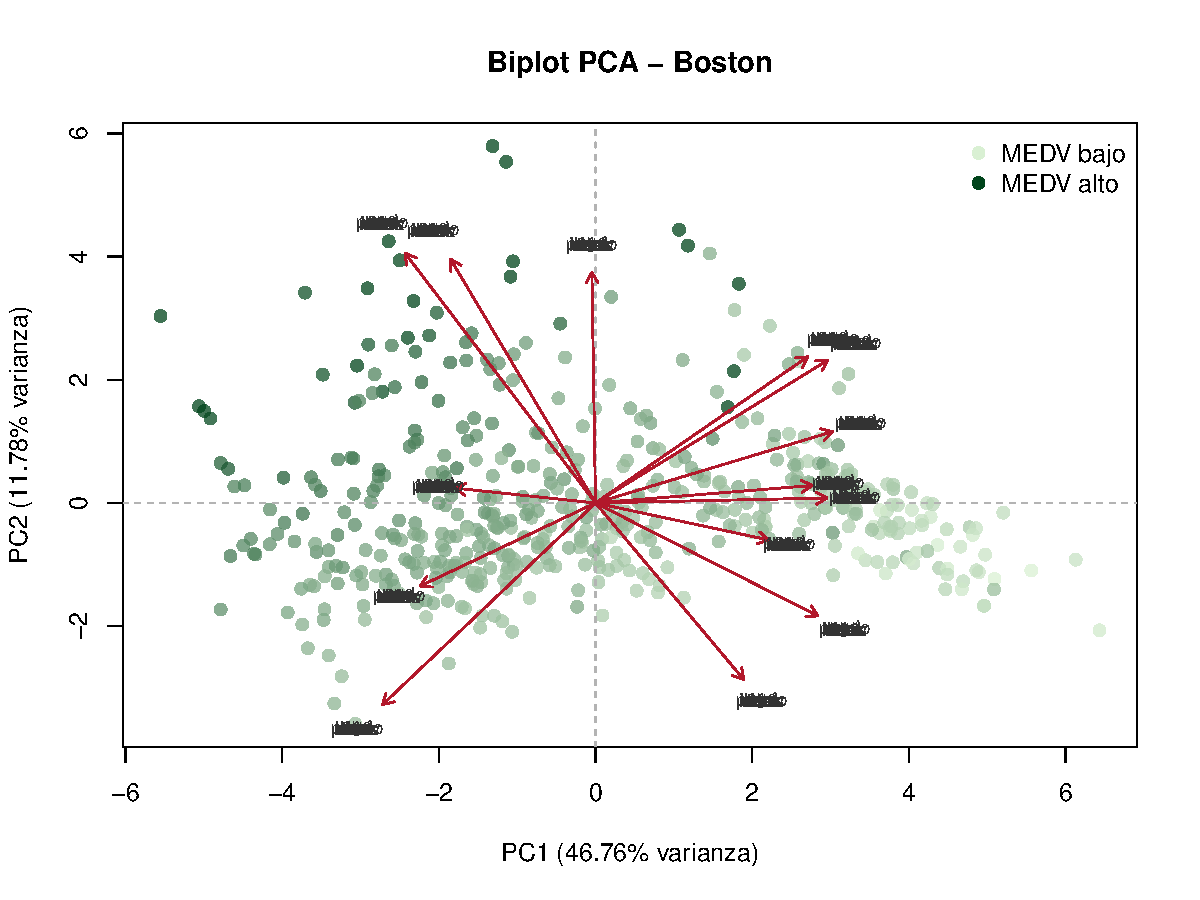
\includegraphics[width=0.82\textwidth]{figuras/fig_08_pca_biplot.pdf}
\caption{Biplot PCA completo con todas las variables del dataset.}
\label{fig:pca_biplot_completo}
\end{figure}

\begin{figure}[H]
\centering
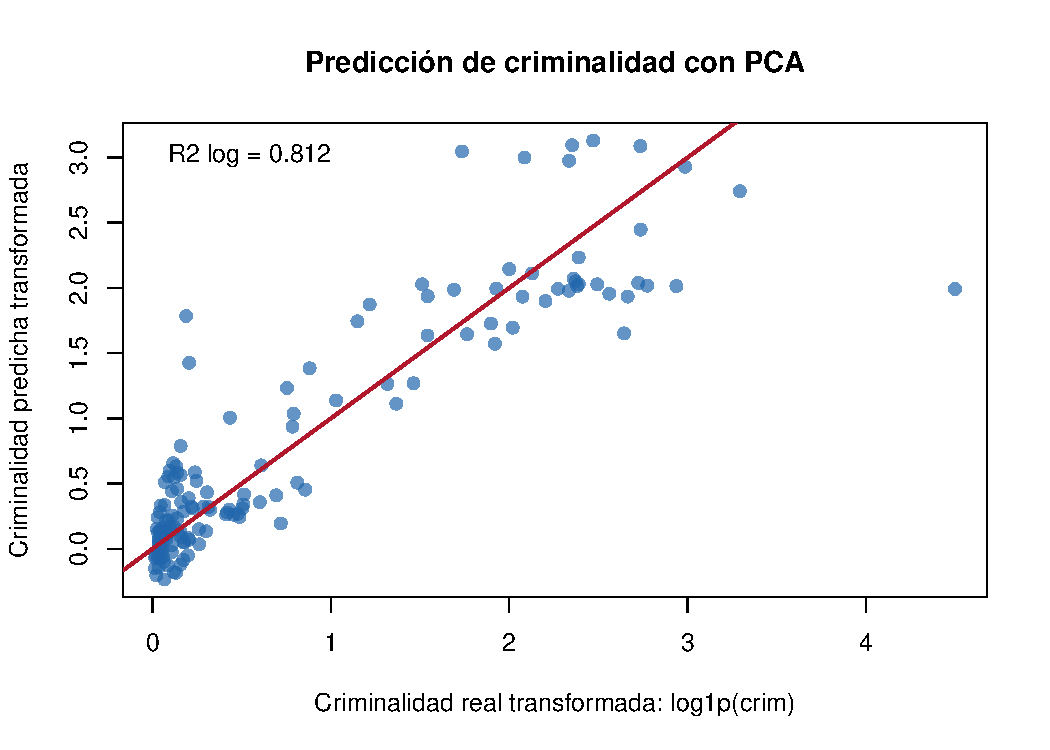
\includegraphics[width=0.72\textwidth]{figuras/fig_09_prediccion_crim.pdf}
\caption{Prediccion de criminalidad transformada mediante regresion sobre componentes principales.}
\label{fig:prediccion_crim}
\end{figure}

\subsection*{A.2 Tablas Complementarias}

\begin{table}[H]
  \centering
  \caption{Resumen descriptivo de variables principales del dataset Boston.}
  \label{tab:resumen_variables}
  \footnotesize
  \begin{tabularx}{\textwidth}{l r r r r r X}
    \toprule
    \textbf{Variable} & \textbf{Media} & \textbf{Mediana} & \textbf{DE} & \textbf{Min.} & \textbf{Max.} & \textbf{Interpretacion} \\
    \midrule
    crim & 3,614 & 0,257 & 8,602 & 0,006 & 88,976 & Criminalidad per capita \\
    rm & 6,285 & 6,208 & 0,703 & 3,561 & 8,780 & Habitaciones promedio \\
    lstat & 12,653 & 11,360 & 7,141 & 1,730 & 37,970 & Menor estatus socioeconomico \\
    medv & 22,533 & 21,200 & 9,197 & 5,000 & 50,000 & Valor mediano de vivienda \\
    tax & 408,237 & 330,000 & 168,537 & 187,000 & 711,000 & Impuesto a la propiedad \\
    ptratio & 18,456 & 19,050 & 2,165 & 12,600 & 22,000 & Ratio alumno-profesor \\
    \bottomrule
  \end{tabularx}
\end{table}

\begin{table}[H]
  \centering
  \caption{Cargas principales de PC1 y PC2 utilizadas para interpretar el PCA.}
  \label{tab:pca_cargas}
  \footnotesize
  \begin{tabularx}{\textwidth}{l X X X}
    \toprule
    \textbf{Componente} & \textbf{Cargas positivas relevantes} & \textbf{Cargas negativas relevantes} & \textbf{Lectura analitica} \\
    \midrule
    PC1 & \texttt{indus}=0,3319; \texttt{nox}=0,3252; \texttt{tax}=0,3240; \texttt{lstat}=0,3114; \texttt{rad}=0,3034 & \texttt{dis}=-0,2982; \texttt{medv}=-0,2666; \texttt{zn}=-0,2454 & Eje de presion urbana/socioeconomica opuesto al valor habitacional. \\
    PC2 & \texttt{medv}=0,4449; \texttt{rm}=0,4340; \texttt{chas}=0,4107; \texttt{age}=0,2603 & \texttt{dis}=-0,3591; \texttt{ptratio}=-0,3146; \texttt{lstat}=-0,2012 & Eje residencial asociado a precio, habitaciones y limite con el rio Charles. \\
    \bottomrule
  \end{tabularx}
\end{table}

\subsection*{A.3 Procedimientos Principales en R}

El codigo completo se encuentra en el archivo \texttt{tarea4\_boston\_pca.R}. A continuacion se muestran los procedimientos principales; el cuerpo del informe no incluye codigo.

\begin{lstlisting}[caption={Carga de datos y revision inicial.}]
library(MASS)
data("Boston", package = "MASS")

boston <- Boston
boston$id_suburbio <- seq_len(nrow(boston))
boston$chas_factor <- factor(boston$chas,
  levels = c(0, 1),
  labels = c("No limita con rio Charles",
             "Limita con rio Charles"))

summary(boston)
colSums(is.na(boston))
\end{lstlisting}

\begin{lstlisting}[caption={PCA sobre variables estandarizadas.}]
vars_analisis <- c("crim", "zn", "indus", "chas", "nox", "rm",
  "age", "dis", "rad", "tax", "ptratio", "black", "lstat", "medv")

pca_data <- boston[, vars_analisis]
pca_boston <- prcomp(pca_data, center = TRUE, scale. = TRUE)

varianza <- pca_boston$sdev^2 / sum(pca_boston$sdev^2)
round(cumsum(varianza) * 100, 2)

cargas <- as.data.frame(pca_boston$rotation[, 1:2])
cargas$abs_PC1 <- abs(cargas$PC1)
cargas$abs_PC2 <- abs(cargas$PC2)
cargas[order(-cargas$abs_PC1), ]
\end{lstlisting}

\begin{lstlisting}[caption={Prediccion de criminalidad con componentes principales.}]
vars_predictoras_crim <- setdiff(vars_analisis, "crim")
idx_train <- sample(seq_len(nrow(boston)), size = floor(0.70 * nrow(boston)))

train <- boston[idx_train, c("crim", vars_predictoras_crim)]
test <- boston[-idx_train, c("crim", vars_predictoras_crim)]

pca_pred <- prcomp(train[, vars_predictoras_crim],
                  center = TRUE, scale. = TRUE)

varianza_pred <- pca_pred$sdev^2 / sum(pca_pred$sdev^2)
n_componentes <- which(cumsum(varianza_pred) >= 0.80)[1]
pc_modelo <- paste0("PC", seq_len(n_componentes))

train_pcs <- as.data.frame(pca_pred$x[, pc_modelo, drop = FALSE])
train_pcs$log_crim <- log1p(train$crim)

test_pcs <- as.data.frame(
  predict(pca_pred, newdata = test[, vars_predictoras_crim])[, pc_modelo]
)

modelo_crim <- lm(log_crim ~ ., data = train_pcs)
pred_log_crim <- predict(modelo_crim, newdata = test_pcs)
\end{lstlisting}

\subsection*{A.4 Bitacora de Trabajo}

\begin{table}[H]
  \centering
  \footnotesize
  \caption{Bitacora de trabajo grupal.}
  \label{tab:bitacora}
  \begin{tabularx}{\textwidth}{l X l}
    \toprule
    \textbf{Fecha} & \textbf{Actividad} & \textbf{Responsable} \\
    \midrule
    Dia 1 & Lectura del enunciado, definicion de preguntas de investigacion y revision de la metodologia CRISP-DM. & Todos \\
    Dia 2 & Carga del dataset Boston, revision de estructura, resumen estadistico, valores faltantes y matriz de correlaciones. & Vicente Rivera \\
    Dia 3 & Deteccion de valores atipicos, analisis de observaciones con menor valor y modelos simples para \texttt{rm}, \texttt{chas} y \texttt{lstat}. & Juan Mu\~noz \\
    Dia 4 & Preparacion de variables, estandarizacion y aplicacion de PCA con interpretacion de varianza y cargas. & Fernando Valdes \\
    Dia 5 & Modelamiento predictivo de criminalidad usando componentes principales y evaluacion con RMSE, MAE y $R^{2}$. & Todos \\
    Dia 6 & Redaccion del informe en LaTeX, integracion de figuras, revision de resultados y preparacion de entrega. & Todos \\
    \bottomrule
  \end{tabularx}
\end{table}

\end{document}
